\documentclass[12pt]{article}
\usepackage[a4paper,left=27mm,right=27mm,top=24mm,bottom=22mm]{geometry}
\usepackage[space]{ctex}
\usepackage{graphicx}
\usepackage{float}
\usepackage{subfigure}
\usepackage{amsmath}
\usepackage{amsfonts,amssymb}
\title{\LARGE\textbf{PossionImageEdit}}
\author{SA21010060 周俊亦}
\date{}

\begin{document}
	\maketitle
	\renewcommand{\abstractname}{Abstract}
	\begin{abstract}
		图像融合是一种十分有趣的图像处理技术应用。本报告复现了经典的图像融合算法: 泊松图像融合(Poisson Image Editing).
	\end{abstract}
	
	\section{算法原理}
		\subsection{概述}
		融合两幅图像的指定区域是十分热门的应用。当然,我们希望图像融合越“自然”越好。如图1所示,如果生硬的剪切图像,这样的融合图像很难达到我们的预期。泊松算法将图像融合看成曲面拟合问题,如图2所示,将剪切图的边缘硬置成背景图像素值,通过调和函数拟合计算生成融合图像。
		
		
		
		\begin{figure}[H]
			\centering
			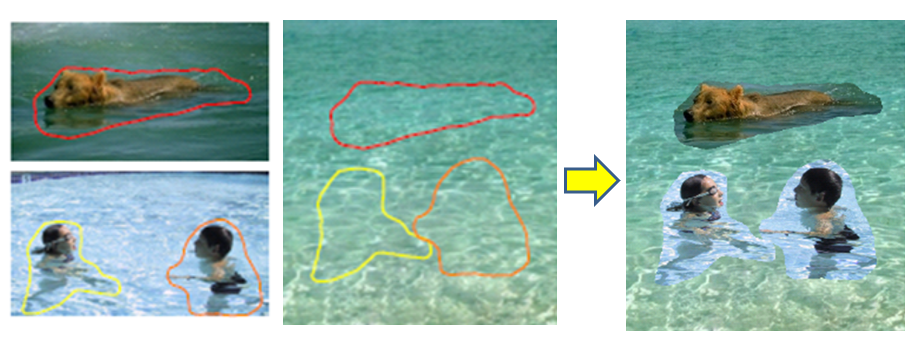
\includegraphics[width=4.1in]{./ppt0.png}
			\centering
			\caption{图像移植}
		\end{figure}
	
	\begin{figure}[H]
		\centering
		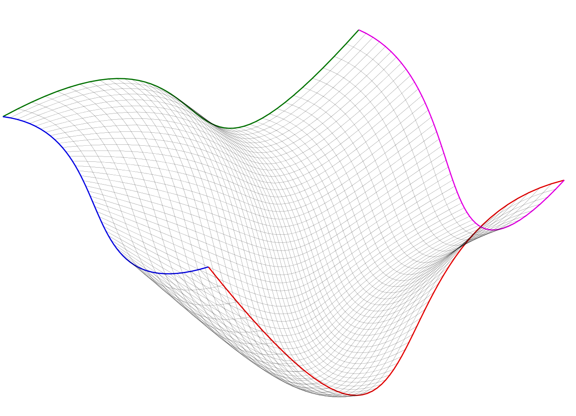
\includegraphics[width=2.7in]{./ppt1.png}
		\centering
		\caption{曲面拟合}
	\end{figure}
	
		\subsection{原理}
		从字面意思上来看,无缝融合(SeamlessCloneing)强调“自然”,尽量让前景(剪切)图与背景图看起来像是原生一起的。自然而然的想法便是让前景图“融入背景图”,这也是前面提到的为什么将前景边缘硬置成背景像素而不是背景边缘硬置成前景像素的原因。
		
		由于融合后必须保留前景的语义,因此,在边缘重置后,需要拟合内部像素,使拟合后的图看起来与原图一致。一般的,图像梯度很大程度上影响了图像的语义,因此,需要让拟合后的图像与原前景图梯度相似。
		
		稍后可知,拟合建模问题是典型的狄利克雷条件下的泊松方程,求解方法可以利用典型的最小二乘。
		
		算法描述为:
		
		给定: 区域$\Omega\in \mathbb{R}^{2}, \Omega \text{上的向量场} \mathbf{v}, \text{以及函数 } f^{*} \in \mathbb{R}^{2}$,求函数 $f$使得:
		$$
		\min _{f} \iint_{\Omega}|\nabla f-\mathbf{v}|^{2} \text { with }\left.f\right|_{\partial \Omega}=f^{*} \mid \partial \Omega
		$$
		
		等价于求解狄利克雷条件下的泊松方程:
		$$
		\Delta f=\operatorname{div} \mathbf{v} \text { over } \Omega, \text { with }\left.f\right|_{\partial \Omega}=\left.f^{*}\right|_{\partial \Omega}
		$$
		
		\begin{figure}[H]
			\centering
			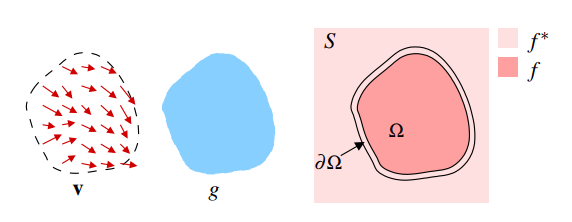
\includegraphics[width=3in]{./paper1.png}
			\centering
			\caption{拟合插值}
		\end{figure}
	
		\subsection{Seamless Cloning}
		连续条件下方程为:
		
		$$
		\min _{\left.f\right|_{\Omega}} \sum_{\langle p, q\rangle \cap \Omega \neq \emptyset}\left(f_{p}-f_{q}-v_{p q}\right)^{2}, \text { with } f_{p}=f_{p}^{*}, \text { for all } p \in \partial \Omega
		$$
		其中:
		
		$N_{p}$为$p$的邻点集,$v_{p q}=\mathbf{v}\left(\frac{p+q}{2}\right) * \overrightarrow{p q}$, 当$\mathbf{v}$是$g$的梯度时,$v_{p q}=g(p)-g(q)$
		
		
		由于图像不是连续函数,需要将上述问题转化为离散条件下的问题:
		
		$$\text{for all\quad} p \in \Omega, \left|N_{p}\right| f_{p}-\sum_{q \in N_{p} \cap \Omega} f_{q}=\sum_{q \in N_{p} \cap \partial \Omega} f_{q}^{*}+\sum_{q \in N_{p}} v_{p q}$$
		
		当 $N_{p} \subset \Omega$ 时:
		
		$$
		\left|N_{p}\right| f_{p}-\sum_{q \in N_{p}} f_{q}=\sum_{q \in N_{p}} v_{p q}
		$$
		
		向量场$\mathbf{v}$的选取方式有多种,这里选取Mixing gradients:
		
		$$
		\text { for all } \mathbf{x} \in \Omega, \mathbf{v}(\mathbf{x})= \begin{cases}\nabla f^{*}(\mathbf{x}) & \text { if }\left|\nabla f^{*}(\mathbf{x})\right|>|\nabla g(\mathbf{x})| \\ \nabla g(\mathbf{x}) & \text { otherwise }\end{cases}
		$$
		
		理论上,该梯度可以自适应前后景梯度。实验验证效果良好。

	\section{实验分析}
	实验使用 Qt5 与 Eigen库 进行算法验证,使用MSVC2017构建生成。
	
		\subsection{程序界面}
	\begin{figure}[H]
		\centering
		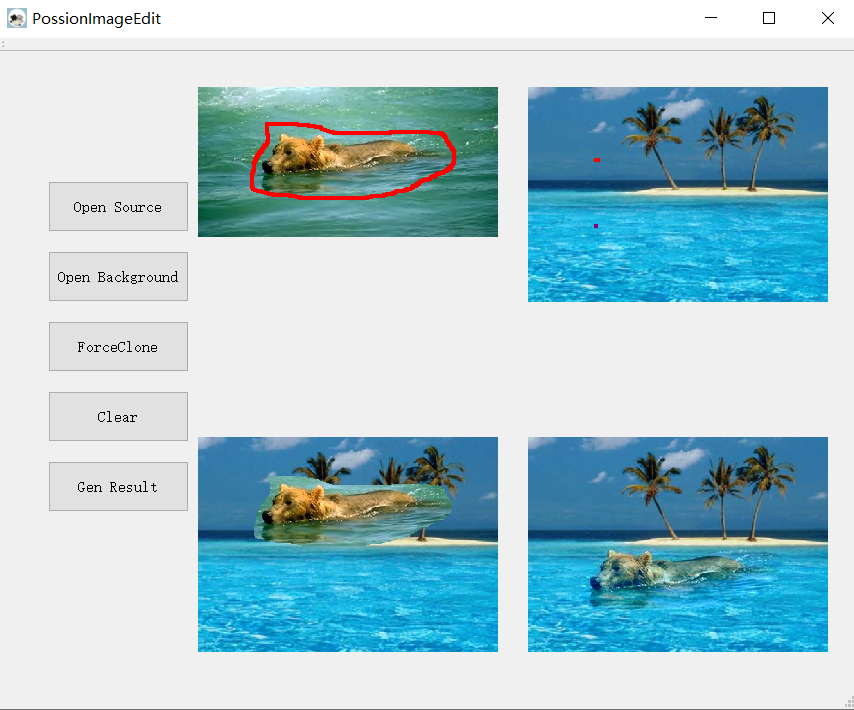
\includegraphics[width=3.7in]{./ui.png}
		\centering
		\caption{程序界面}
	\end{figure}
	
	如图,程序可以实现任意曲线的图像融合,点击暴力融合按键可以查看暴力融合的预览, 在右上角目标图像设置位移矢量的起点(左键描点)与终点(右键描点)可以改变前景与背景融合的位置。
	
	\subsection{Examples}
	
		\begin{figure}[H]
			\centering
			\subfigure[source]{
				\begin{minipage}[t]{0.3\linewidth}
					\centering
					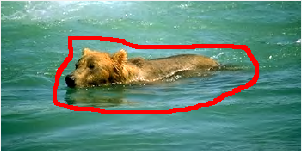
\includegraphics[width=1.7in]{./s1.png}
					%\caption{fig1}
				\end{minipage}%
			}%
			\subfigure[target]{
				\begin{minipage}[t]{0.3\linewidth}
					\centering
					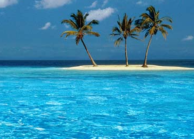
\includegraphics[width=1.7in]{./ocean2.png}
					%\caption{fig2}
				\end{minipage}%
			}
			\subfigure[result]{
				\begin{minipage}[t]{0.3\linewidth}
					\centering
					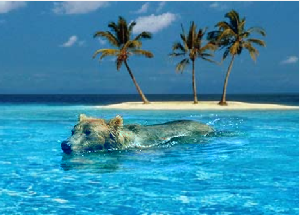
\includegraphics[width=1.7in]{./r1.png}
					%\caption{fig2}
				\end{minipage}%
			}
			\centering
			\caption{Ex1.}
		\end{figure}
		
		\begin{figure}[H]
			\centering
			\subfigure[source]{
				\begin{minipage}[t]{0.3\linewidth}
					\centering
					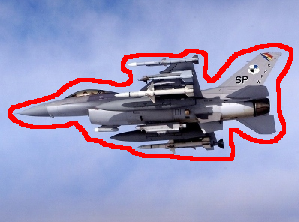
\includegraphics[width=1.7in]{./s2.png}
					%\caption{fig1}
				\end{minipage}%
			}%
			\subfigure[target]{
				\begin{minipage}[t]{0.3\linewidth}
					\centering
					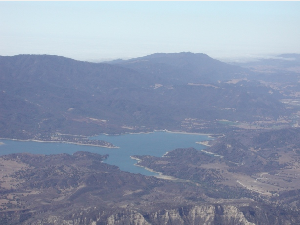
\includegraphics[width=1.7in]{./b2.png}
					%\caption{fig2}
				\end{minipage}%
			}
			\subfigure[result]{
				\begin{minipage}[t]{0.3\linewidth}
					\centering
					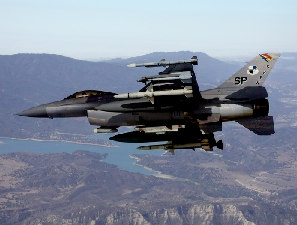
\includegraphics[width=1.7in]{./r2.png}
					%\caption{fig2}
				\end{minipage}%
			}
			\centering
			\caption{Ex2.}
		\end{figure}
		
		\begin{figure}[H]
			\centering
			\subfigure[source]{
				\begin{minipage}[t]{0.3\linewidth}
					\centering
					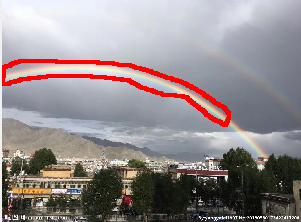
\includegraphics[width=1.7in]{./s3.png}
					%\caption{fig1}
				\end{minipage}%
			}%
			\subfigure[target]{
				\begin{minipage}[t]{0.3\linewidth}
					\centering
					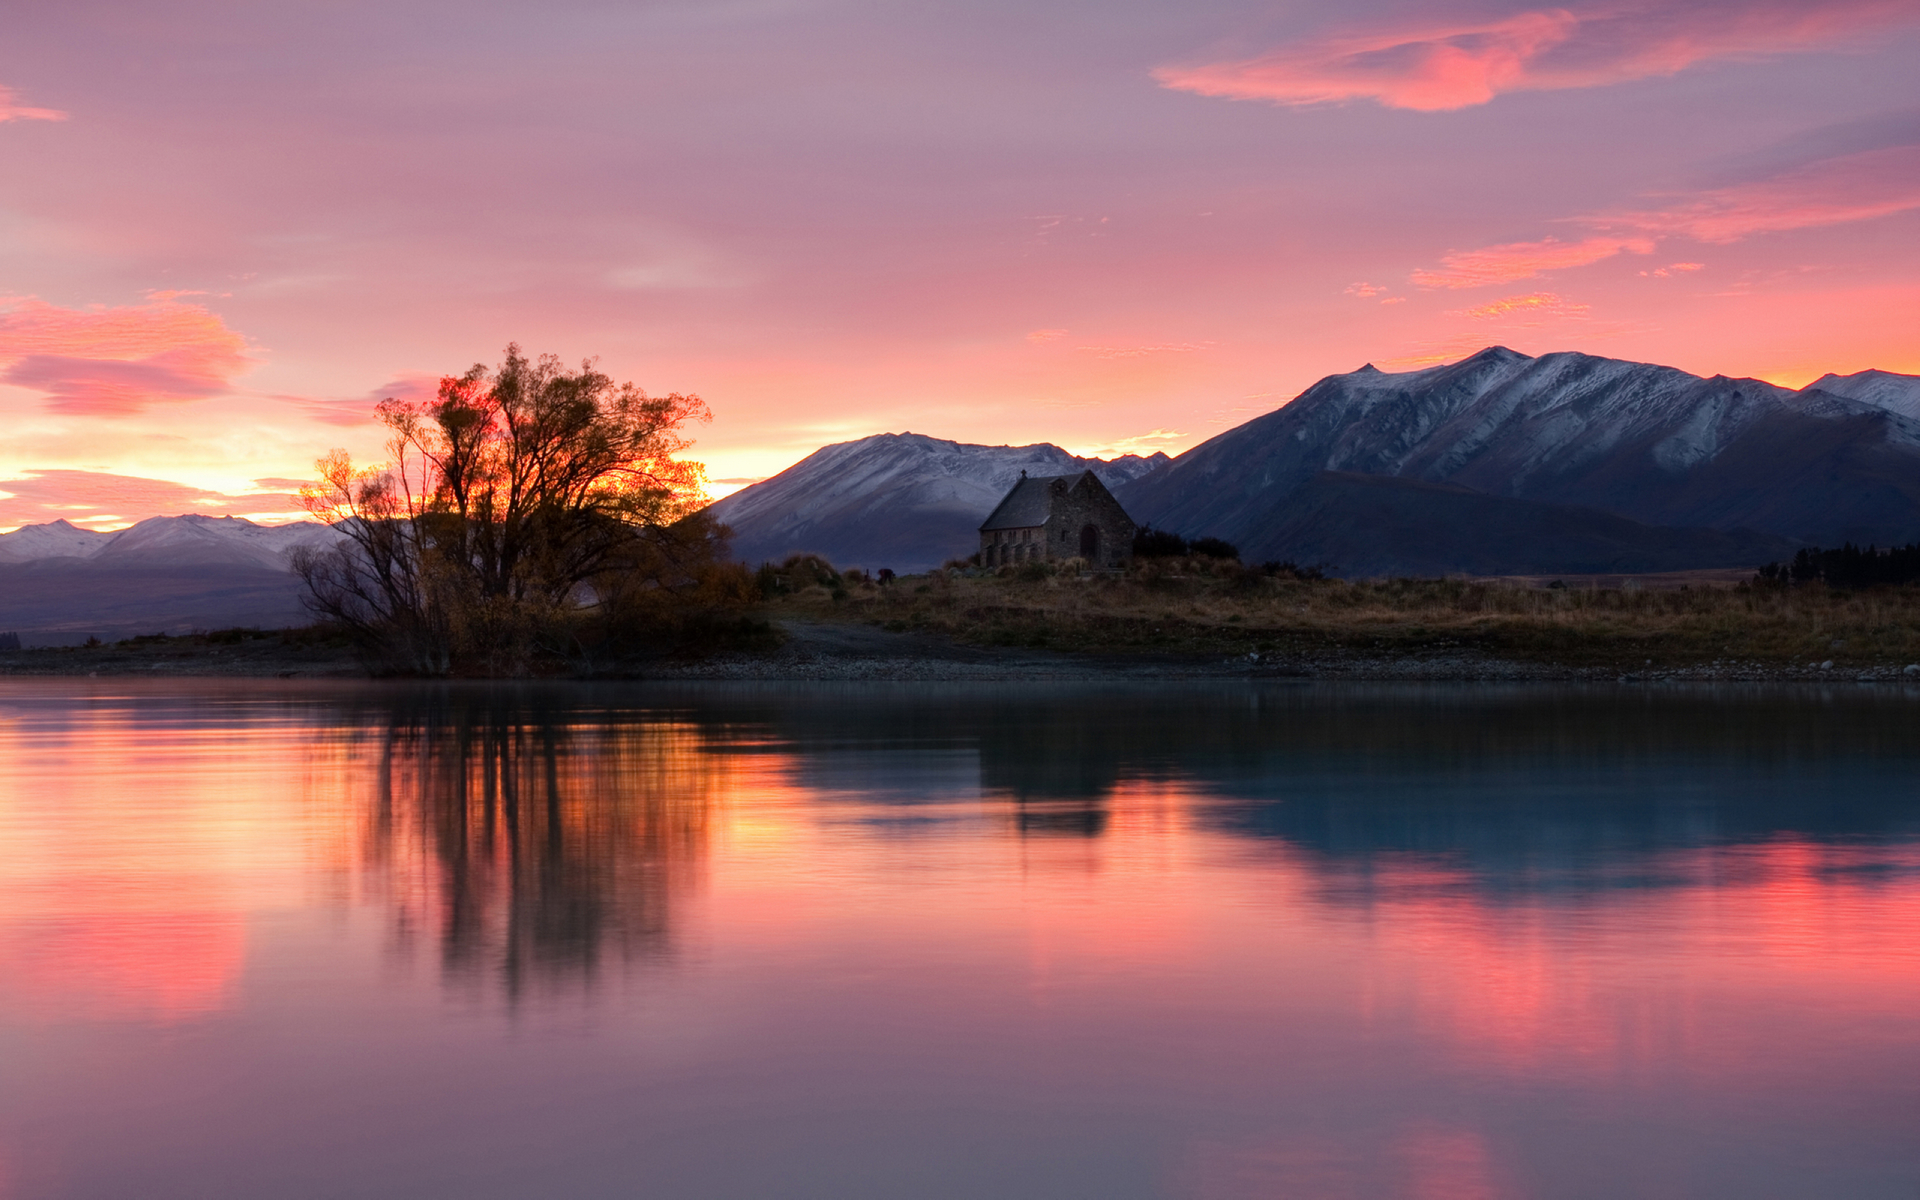
\includegraphics[width=1.7in]{./b3.jpg}
					%\caption{fig2}
				\end{minipage}%
			}
			\subfigure[result]{
				\begin{minipage}[t]{0.3\linewidth}
					\centering
					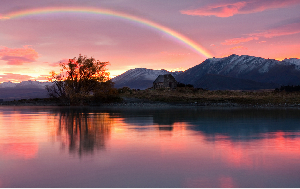
\includegraphics[width=1.7in]{./r3_1.png}
					%\caption{fig2}
				\end{minipage}%
			}
			\centering
			\caption{Ex3. So beautiful !!!}
		\end{figure}
	
	实验中求解大型稀疏方阵时使用Cholesky分解,极大的提高了方程的解的速度,比BiCGSTAB约快两个数量级。\\
	
	
	实验中发现程序运行耗时主要在生成稀疏矩阵的过程里,推测可能是Eigen的稀疏矩阵的插入耗时。图8显示了Example2的运行时长截图。可以发现,方程求解是很快的。
	
	\begin{figure}[H]
		\centering
		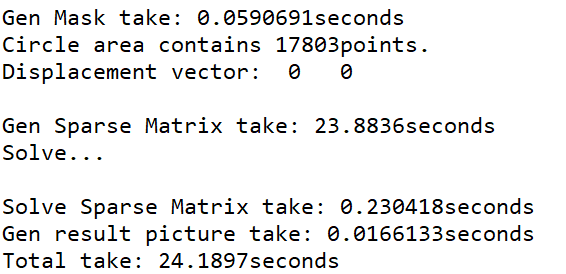
\includegraphics[width=3.7in]{./time.png}
		\centering
		\caption{running time}
	\end{figure}

	\section{实验总结}
	又是大开眼界的一次应用实践。本次实验复现了图像融合算法,在应用中进一步体会到了数学的奇妙。
	
	附睿客网代码链接:https://rec.ustc.edu.cn/share/8ab70680-3a56-11ec-b63a-414d96e82c31
	
	\begin{thebibliography}{99}
	
		\bibitem{1}Patrick Pérez, Michel Gangnet, and Andrew Blake. 2003. Poisson image editing. ACM Trans. Graph. 22, 3 (July 2003), 313–318. 
		
	\end{thebibliography}
\end{document}

